\newpage
\section{Vector Space Retrieval Model}

VSM - Vector Space Model

%----------------------------------------
\subsection{Vector Space Model (VSM): Illustration}

\begin{figure}[H]
    \centering
    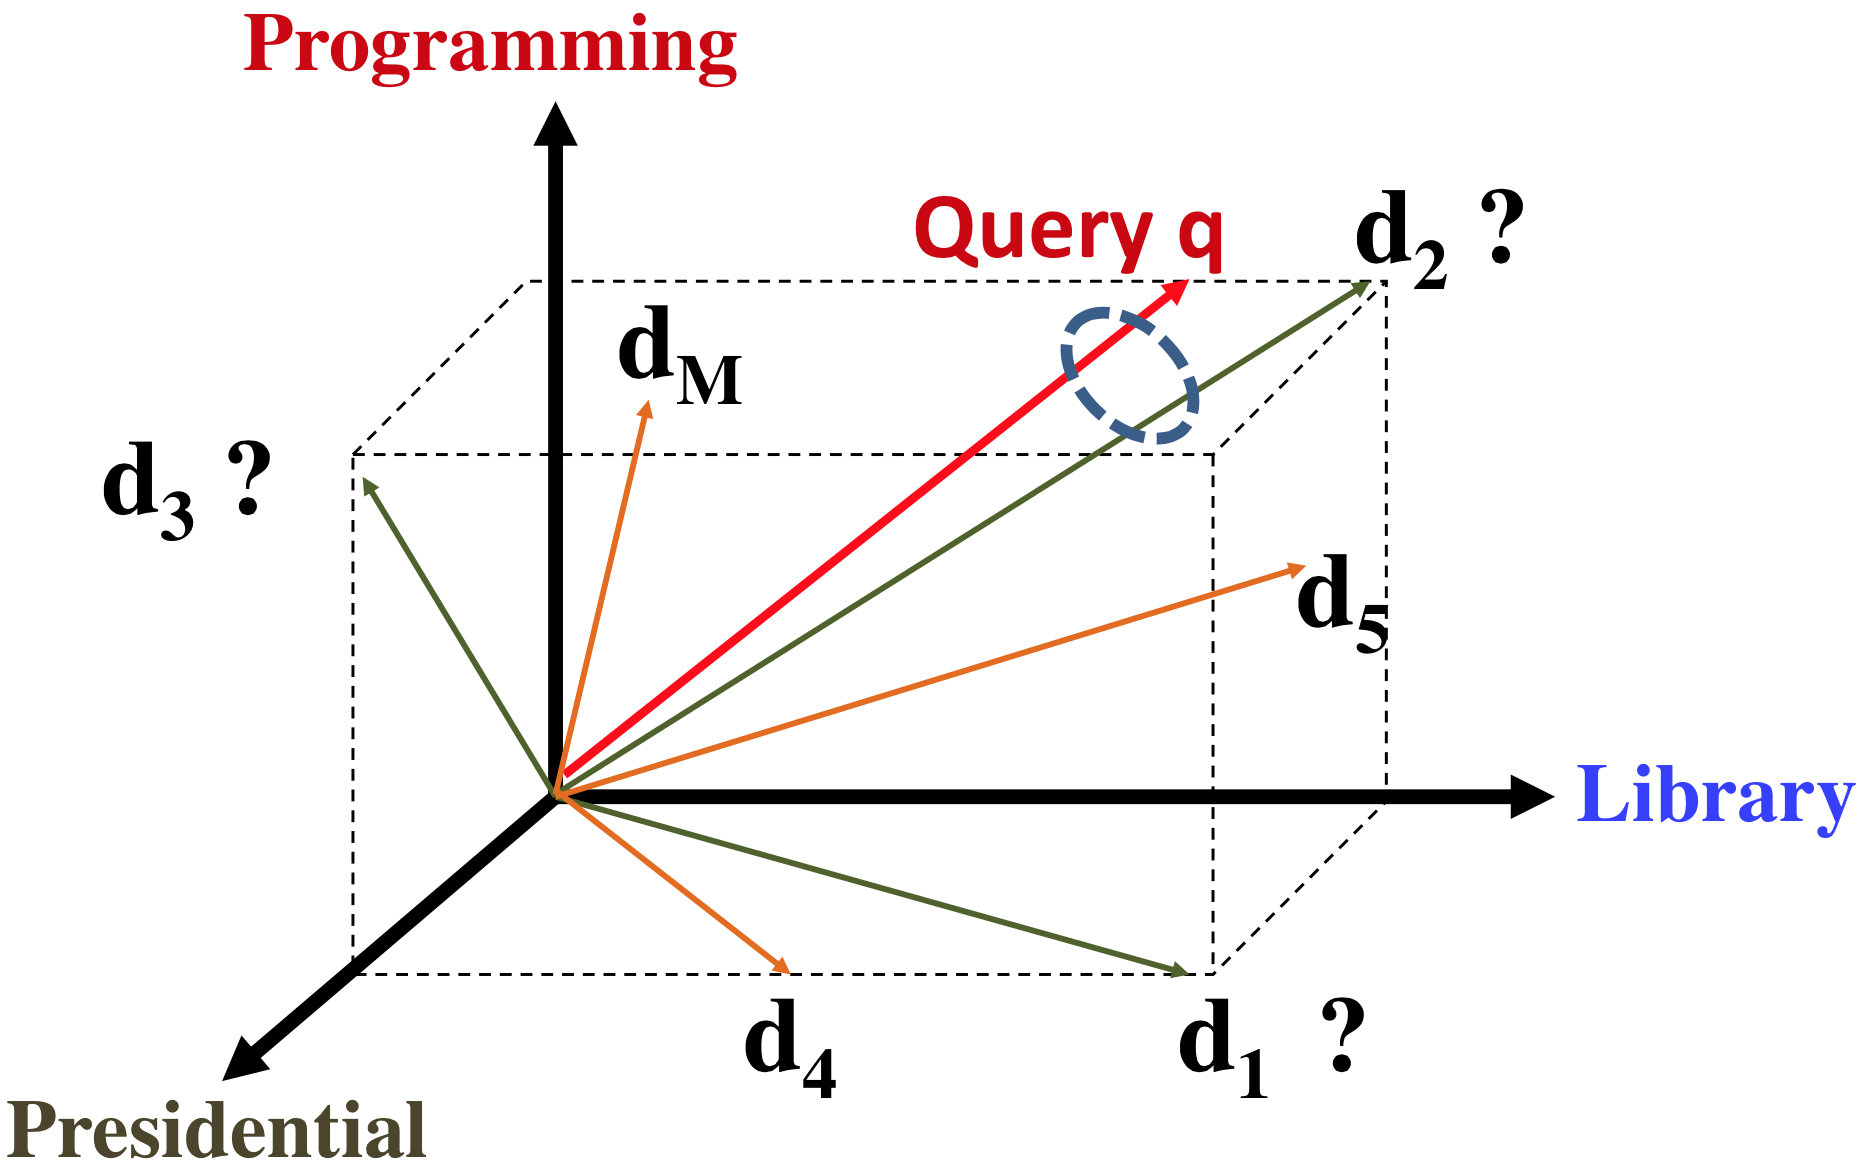
\includegraphics[width=0.9\linewidth]{VSM.png}
\end{figure}

%----------------------------------------
\subsection{VSM Is a Framework}
\begin{itemize}
\item Represent a doc/query by a term vector
\begin{itemize}
\item \textbf{Term}: basic concept, e.g., word or phrase
\item Each term defines one dimension
\item N terms define an \textbf{N-dimensional space}
\item \textbf{Query vector}: $q=(x_1, \dots x_N), x_i \in \Re$ is query term weight 
\item \textbf{Doc} vector: $d=(y_1, \dots y_N), y_j \in \Re$ is doc term weight
\end{itemize}
\item $relevance(q,d) \propto similarity(q,d)=f(q,d)$
\end{itemize}


%----------------------------------------
\subsection{What VSM Doesn’t Say}
\begin{itemize}
\item How to define/select the “basic concept” – Concepts are assumed to be orthogonal
\item How to place docs and query in the space (= how to assign term weights)

\begin{itemize}
\item Term weight in query indicates importance of term 
\item Term weight in doc indicates how well the term characterizes the doc
\end{itemize}

\item How to define the similarity measure
\end{itemize}


\begin{figure}[H]
    \centering
    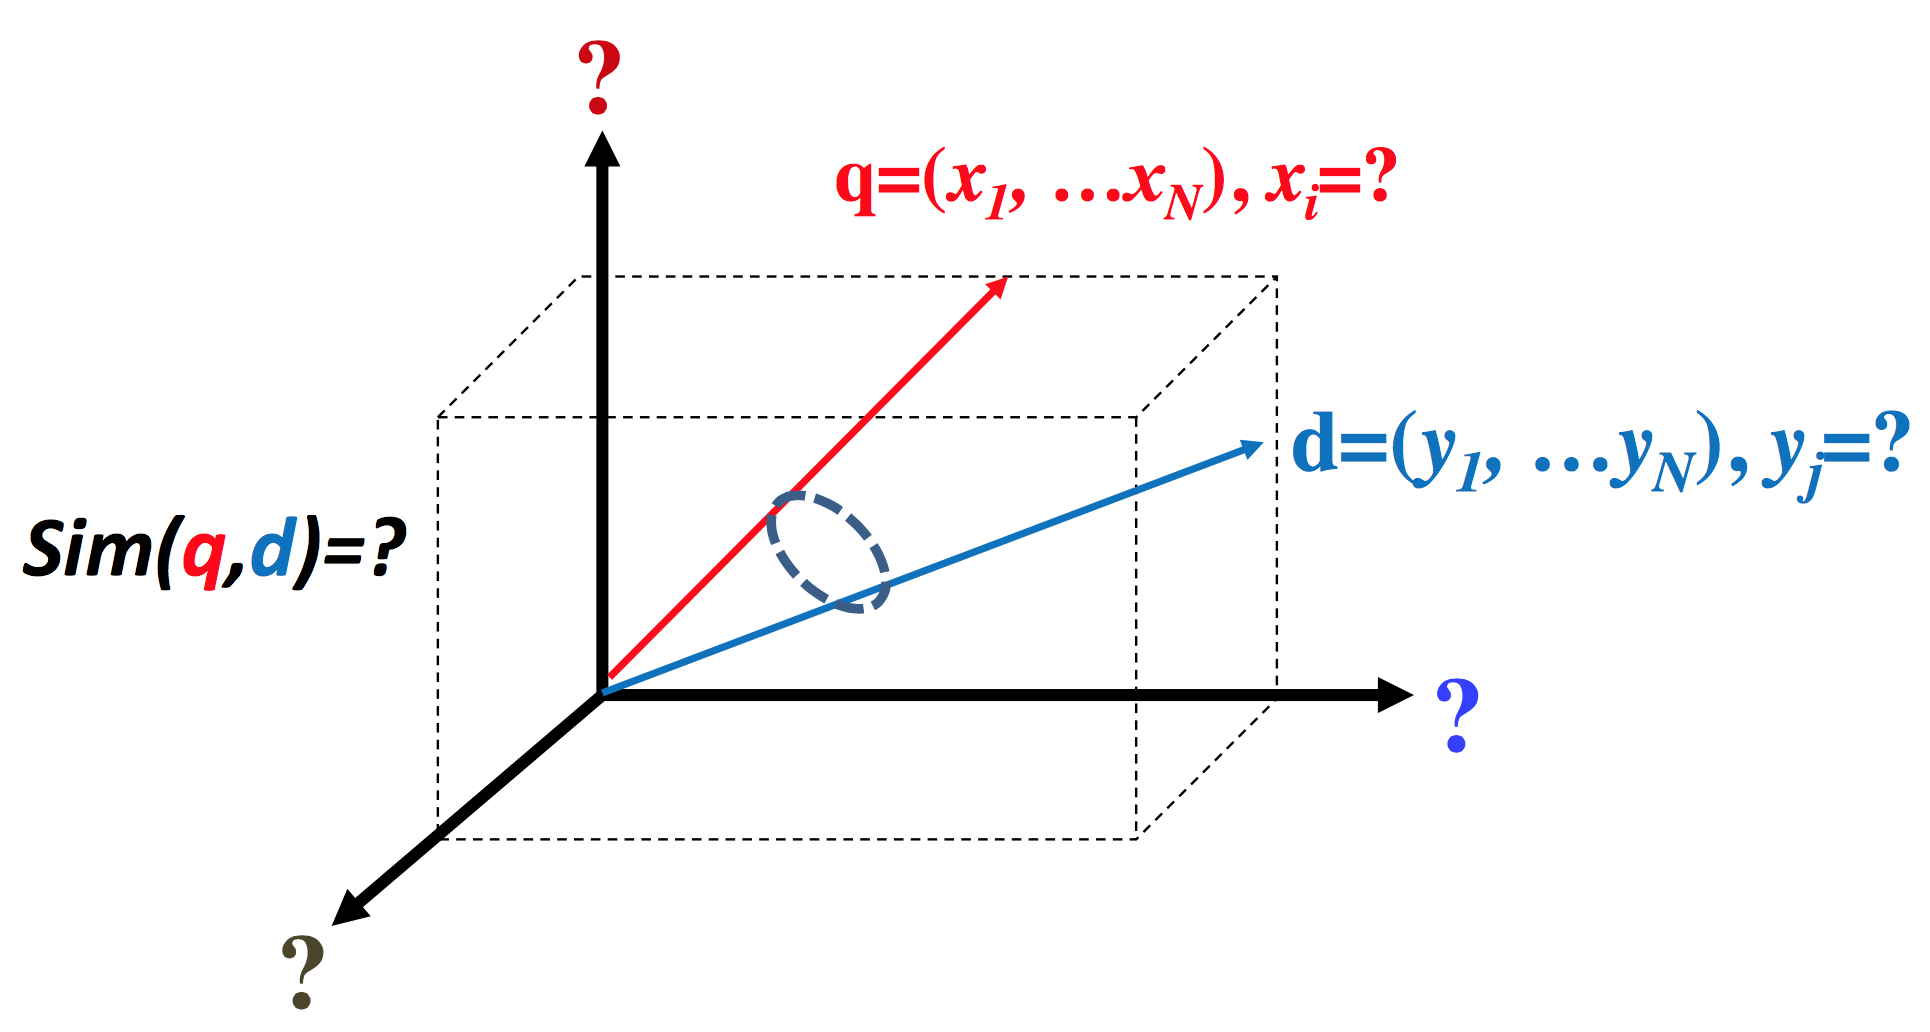
\includegraphics[width=\linewidth]{vsm_questions.png}
\end{figure}


%----------------------------------------
\subsection{Simplest VSM = Bit-Vector + Dot-Product + BOW}
\begin{figure}[H]
    \centering
    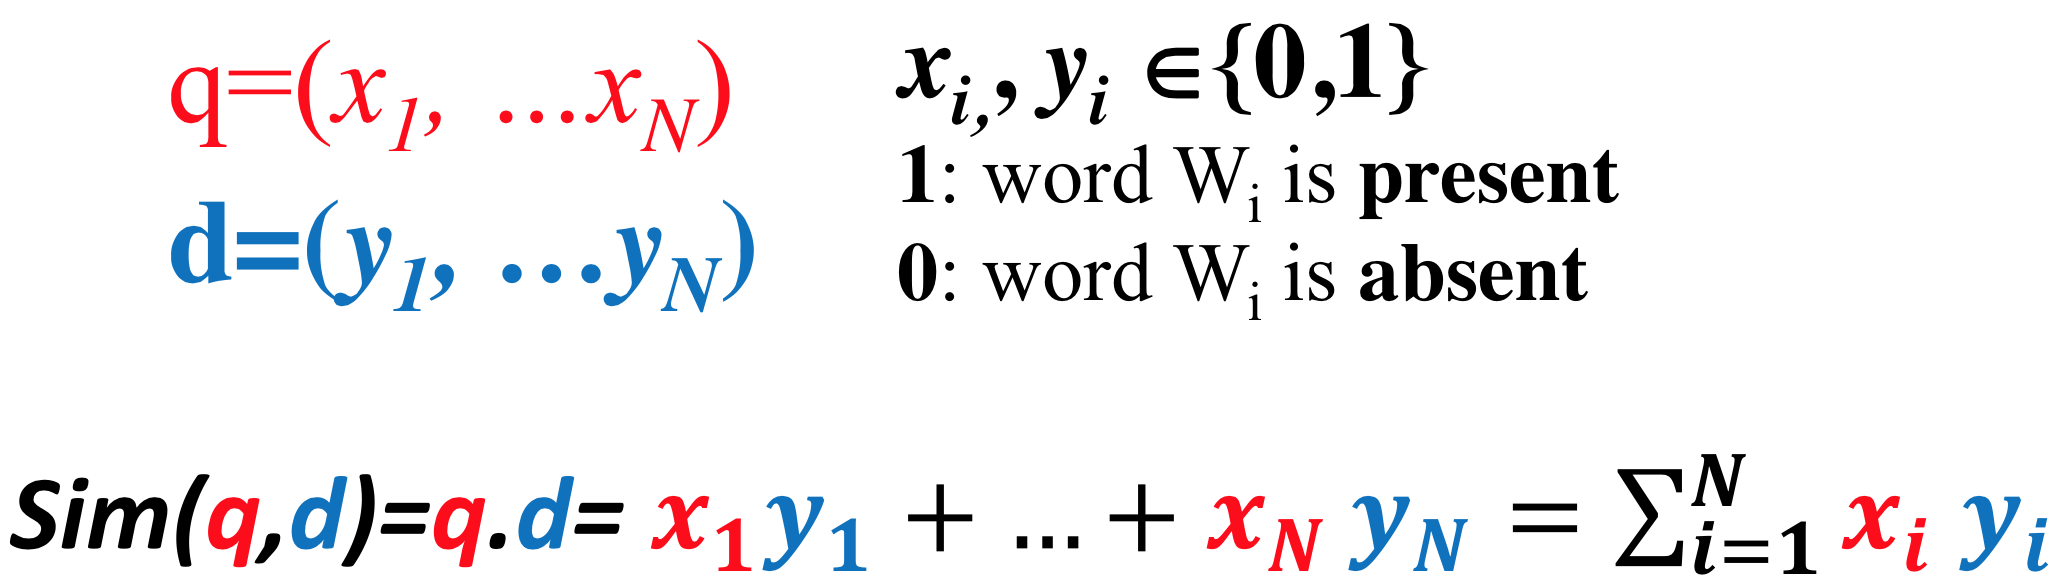
\includegraphics[width=\linewidth]{simplest_vsm.png}
\end{figure}

Simplest VSM:
\begin{itemize}
\item Dimension = word
\item Vector = 0-1 bit vector (word presence/absence)
\item Similarity = dot product
\item f(q,d) = number of distinct query words matched in d
\end{itemize}


%----------------------------------------
\subsection{Improved Instantiation}

Improved VSM:
\begin{itemize}
\item Dimension = word
\item Vector = TF-IDF weight vector
\item Similarity = dot product
\end{itemize}

%----------------------------------------
\subsection{Improved VSM with Term Frequency (TF) Weighting}
\begin{figure}[H]
    \centering
    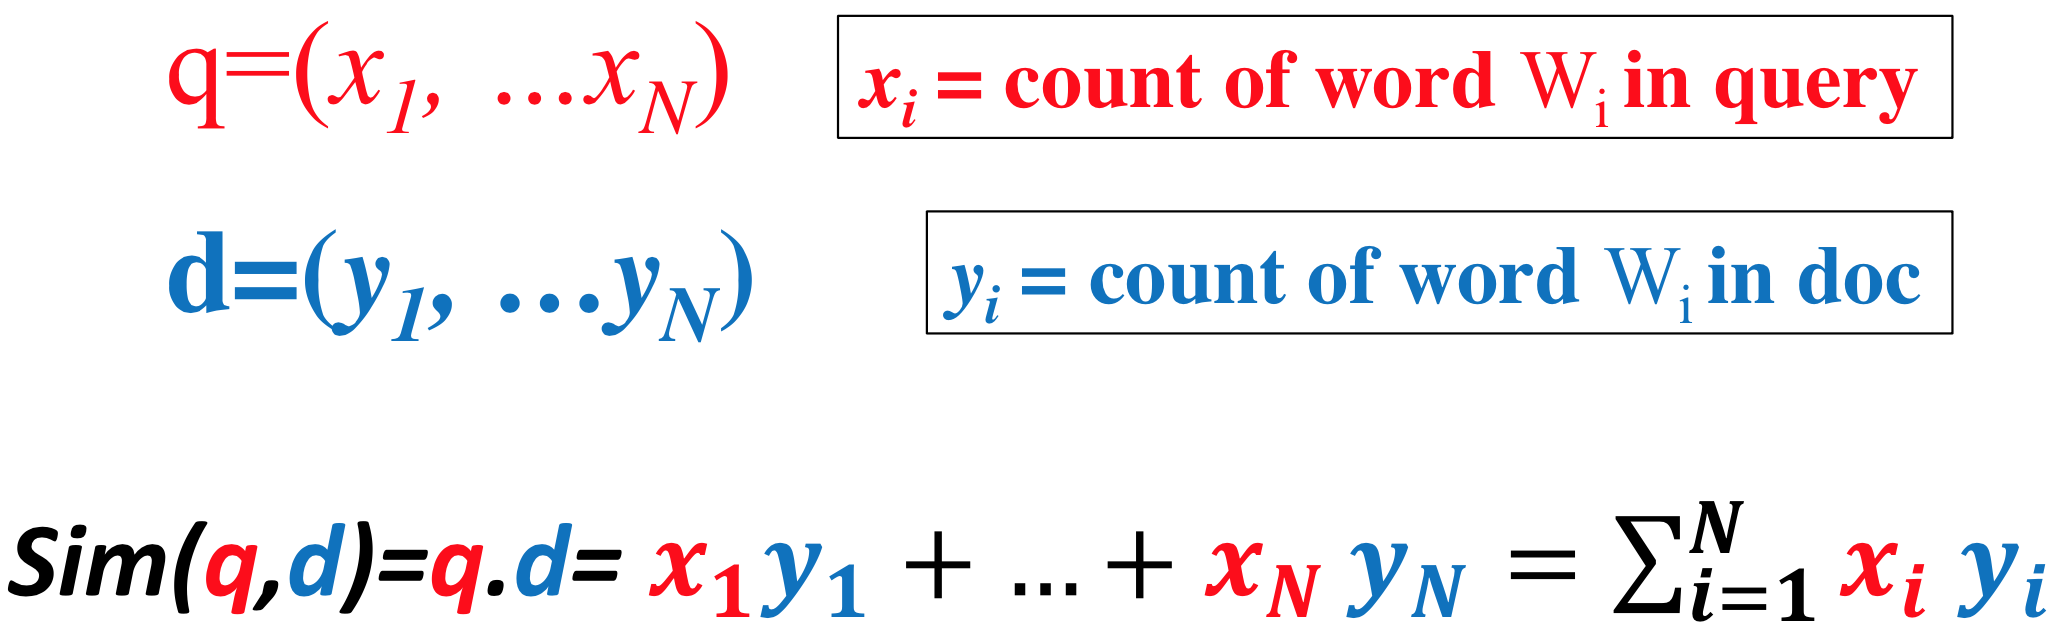
\includegraphics[width=0.6\linewidth]{VSM_TF.png}
\end{figure}

%----------------------------------------
\subsection{IDF Weighting: Penalizing Popular Terms}
IDF — inverse document frequency
\begin{figure}[H]
    \centering
    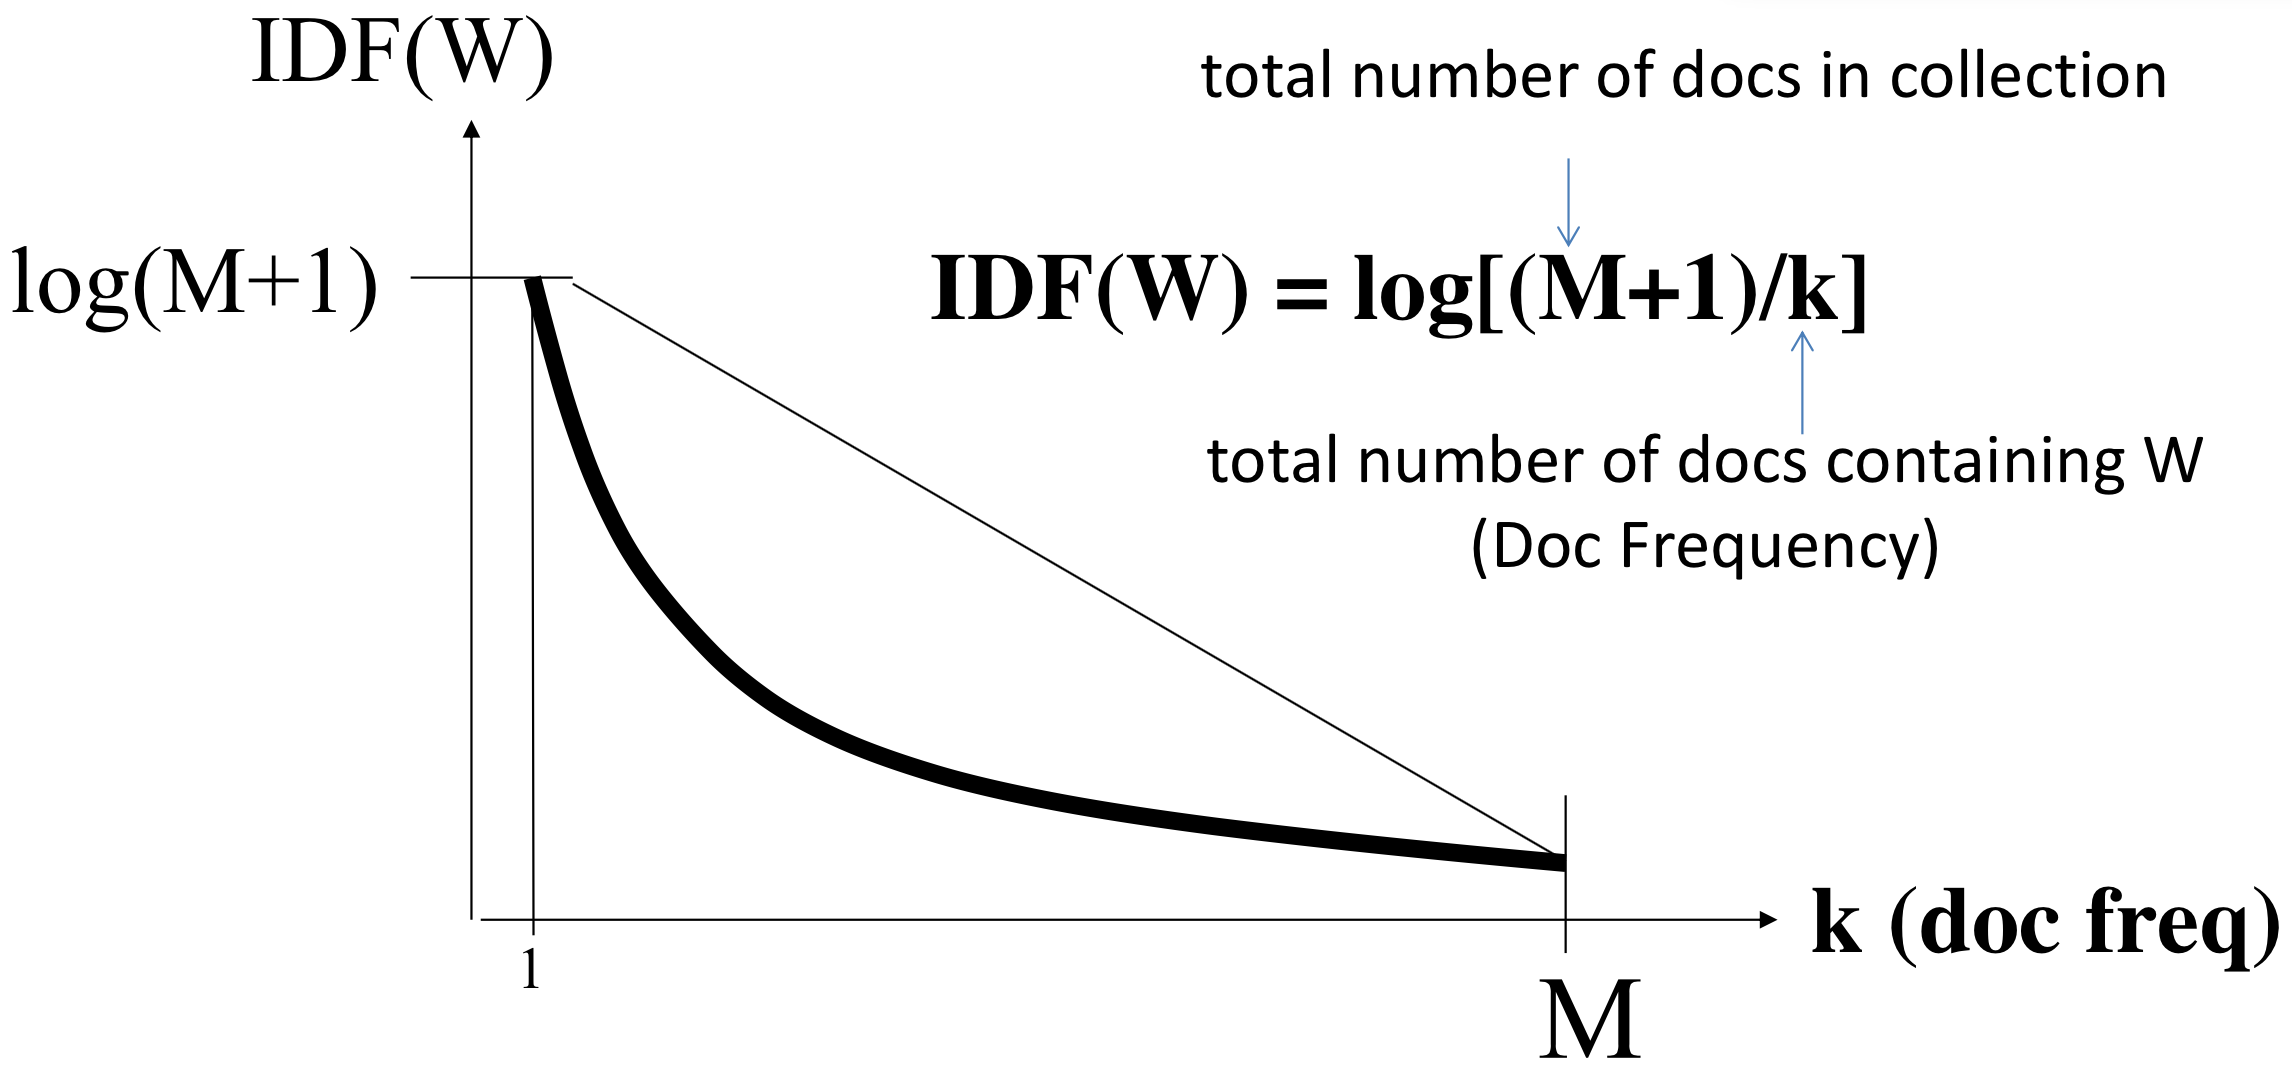
\includegraphics[width=0.85\linewidth]{IDF.png}
\end{figure}

%----------------------------------------
\subsection{Adding Inverse Document Frequency (IDF)}
\begin{figure}[H]
    \centering
    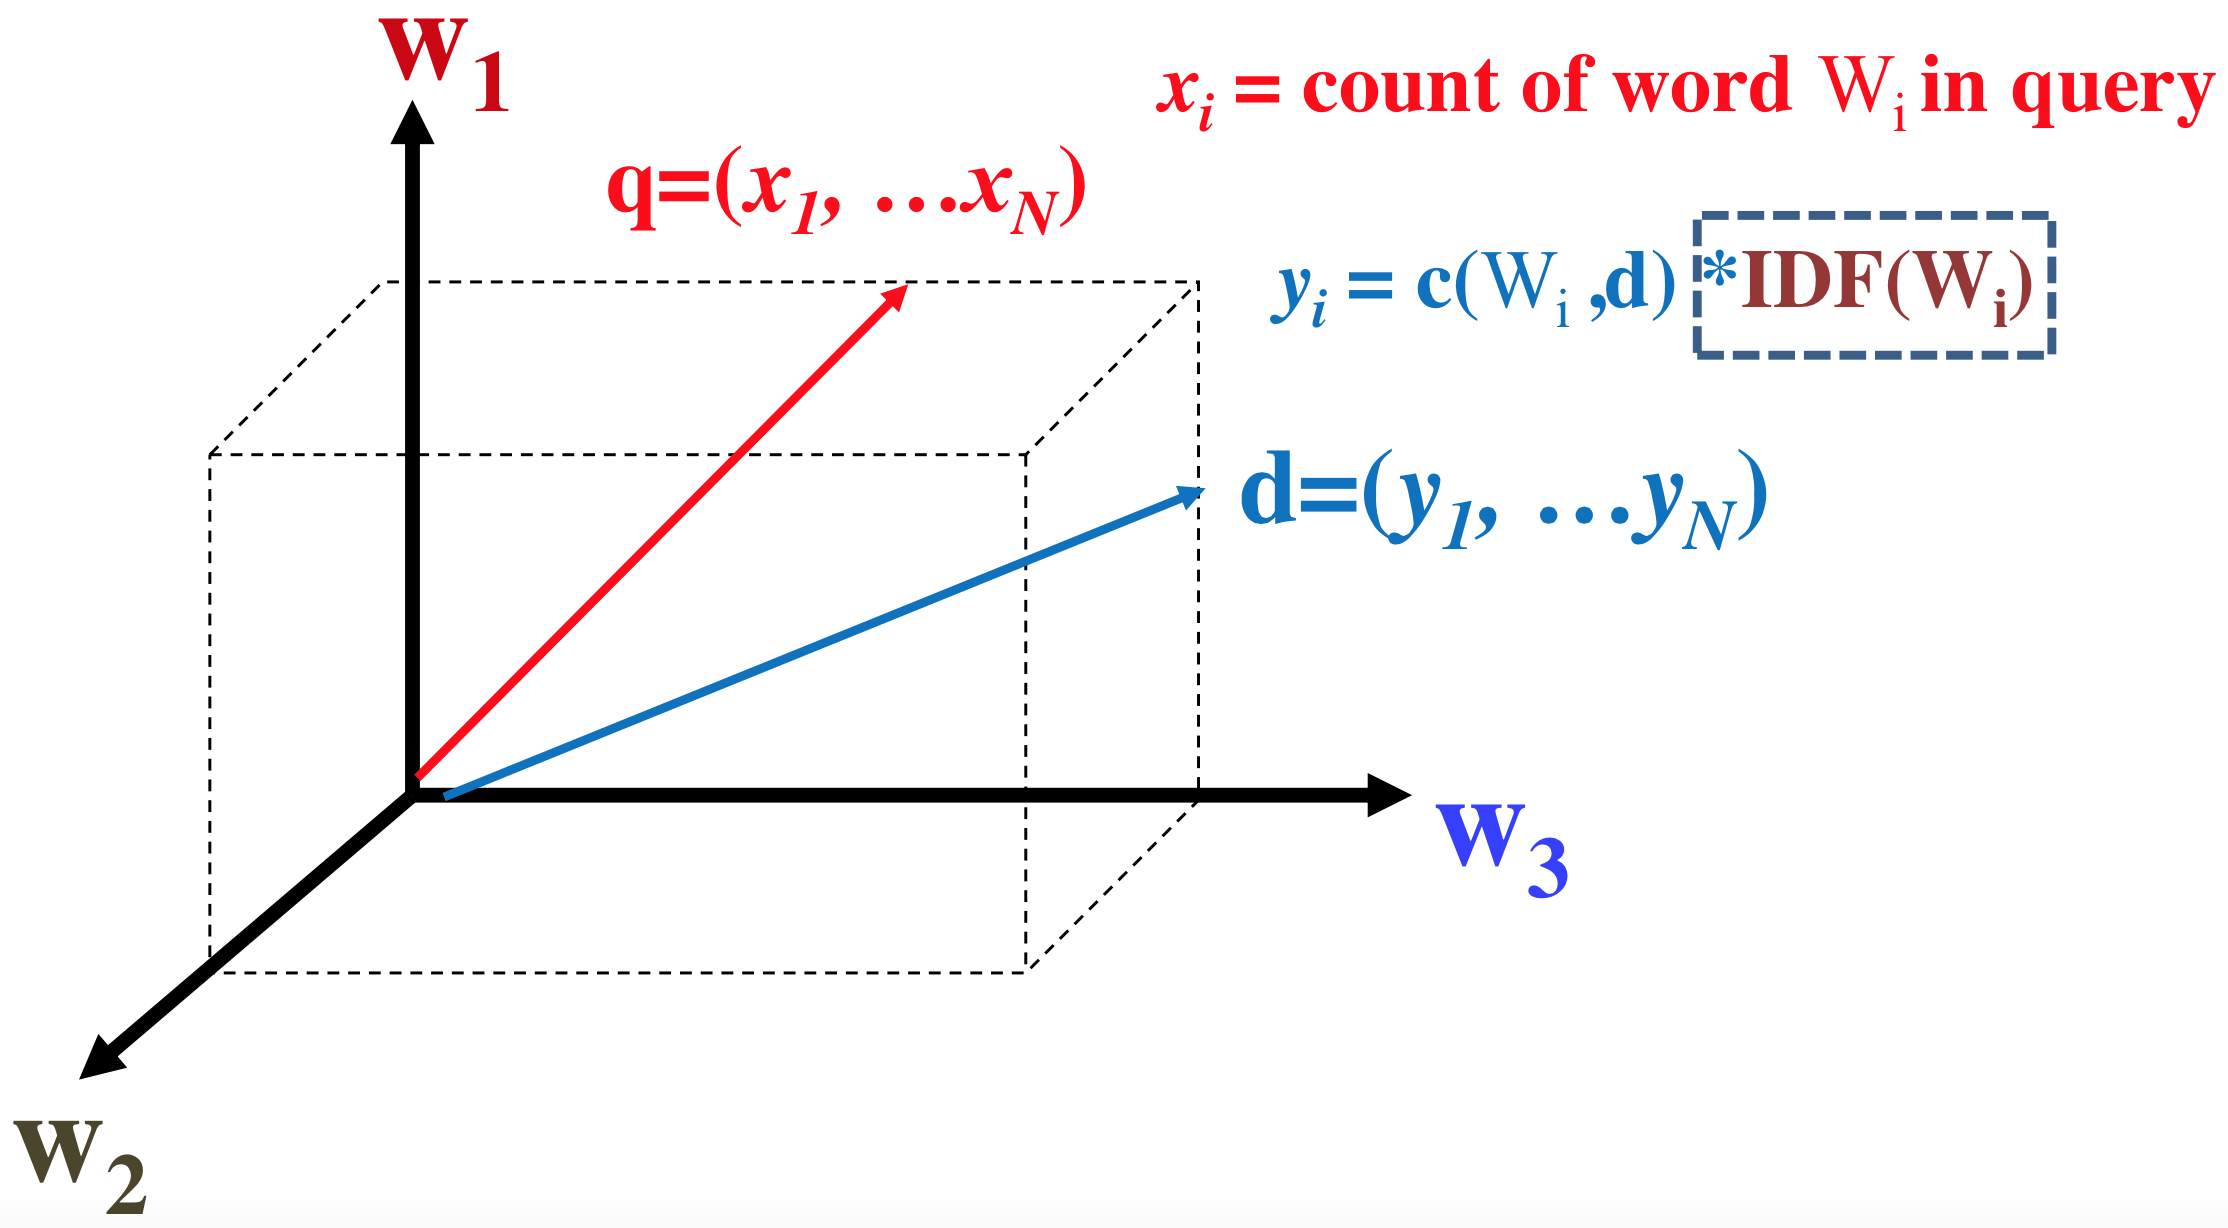
\includegraphics[width=0.85\linewidth]{VSM_IDF.png}
\end{figure}


%----------------------------------------
\subsection{Ranking Function with TF-IDF Weighting}

\begin{equation*}
f(q, d) = \sum_{i=1}^N x_i \, y_i = \sum_{w \in q \cap d} c(w, q) \: c(w, d) \log \frac{M+1}{df(w)}
\end{equation*}

\begin{itemize}
\item $w \in q \cap d$ - all matched query (q) words in document (d)
\item $c(w, q)$ - count of word w in document d
\item $M$ - total number of documents in collection
\item $df(w)$ - Doc Frequency (total number of documents containing word w)
\end{itemize}

%\begin{figure}[H]
%    \centering
%    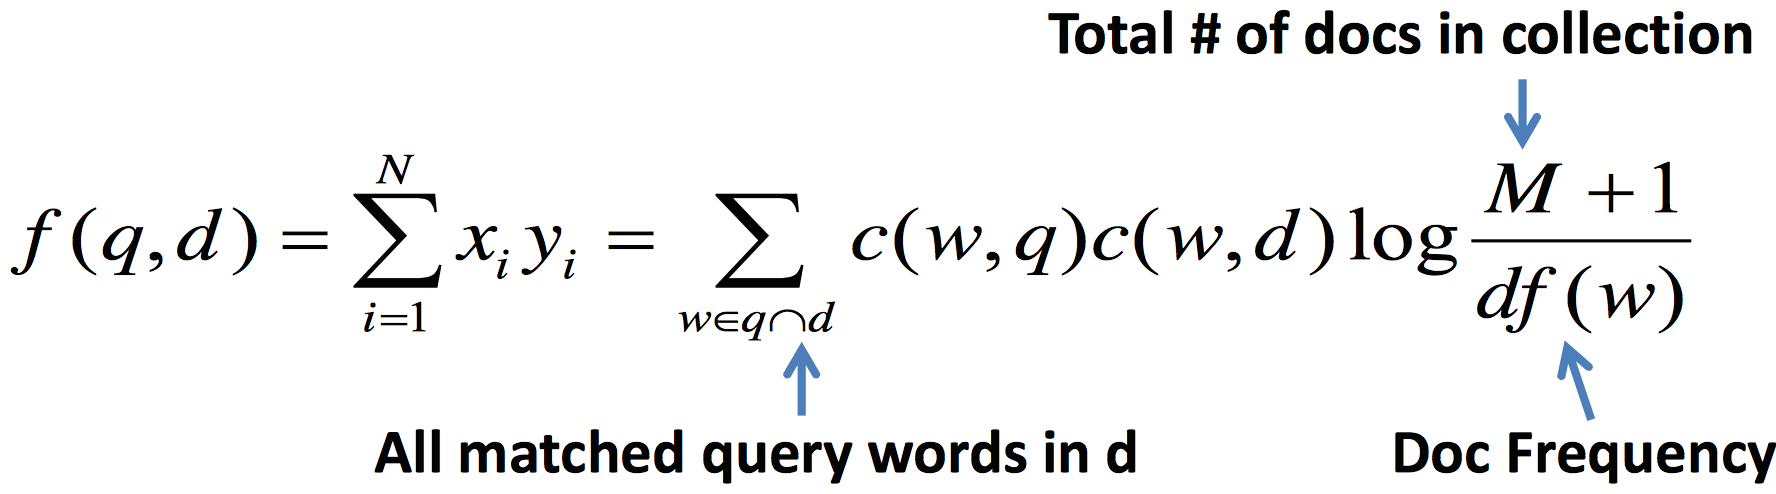
\includegraphics[width=\linewidth]{TF_IDF.png}
%\end{figure}


%----------------------------------------
\subsection{TF Transformation: BM25 Transformation}
BM = Best Matching

\begin{figure}[H]
    \centering
    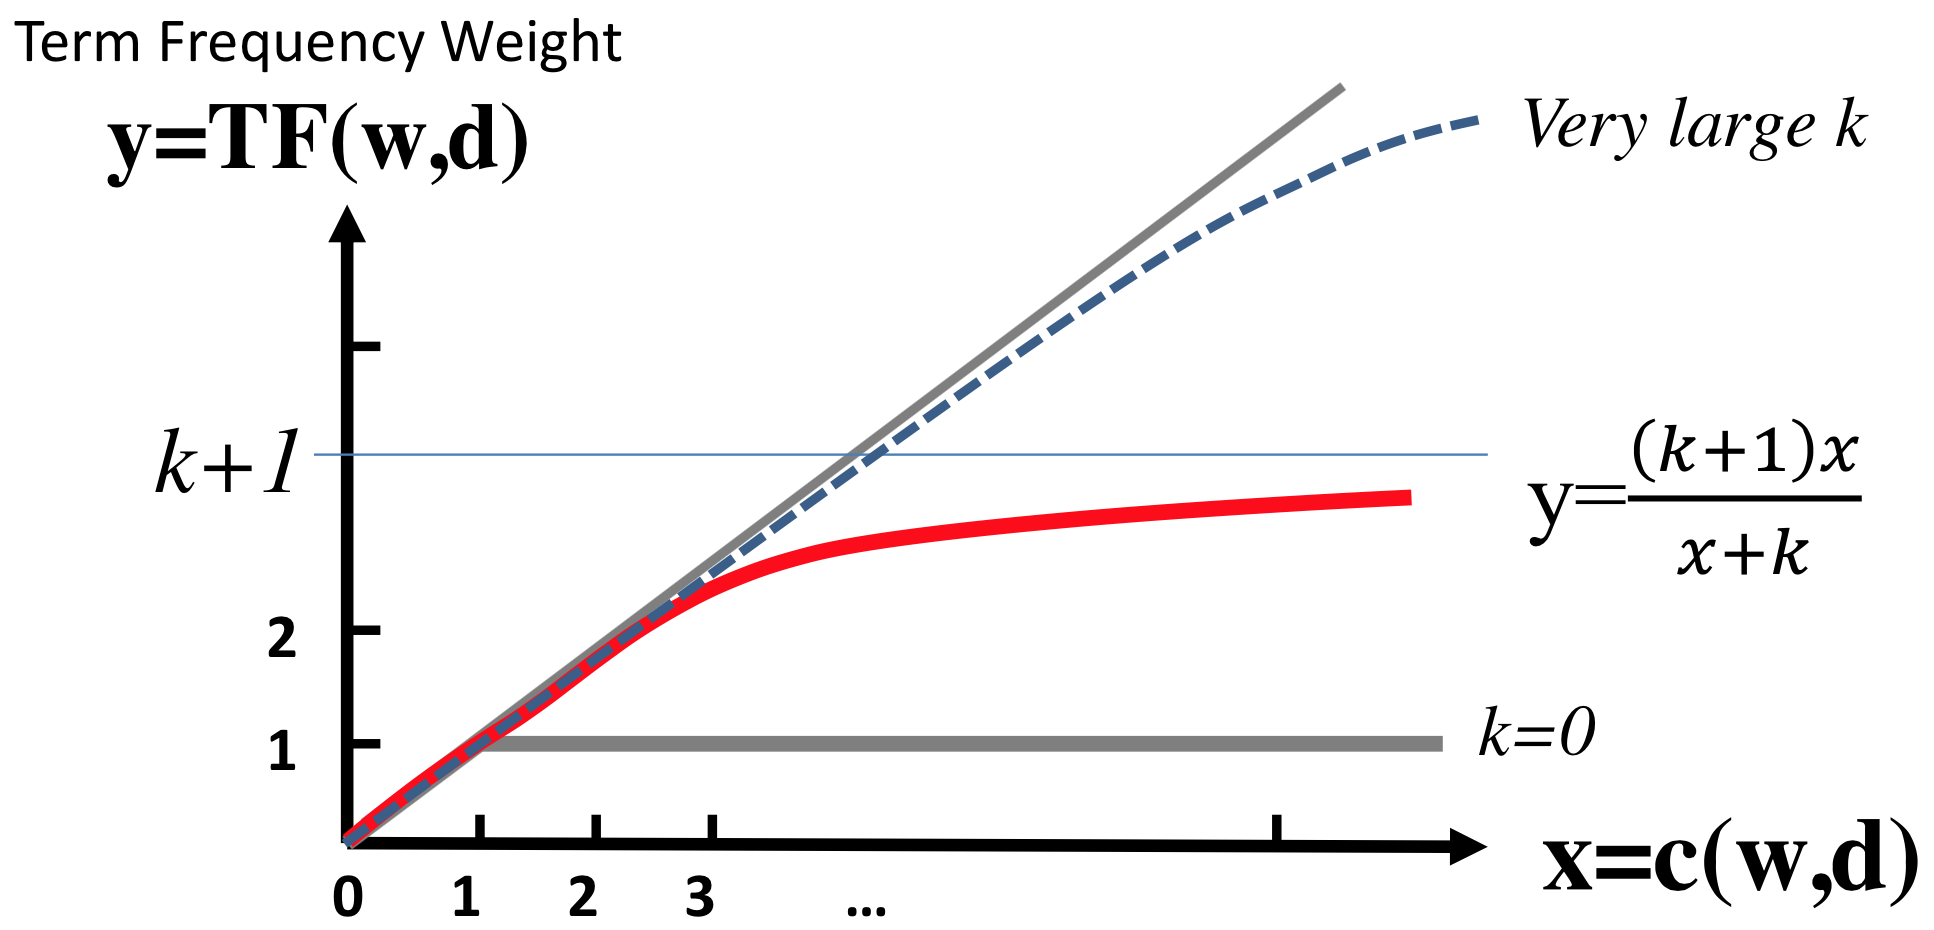
\includegraphics[width=0.75\linewidth]{BM25_transformation.png}
\end{figure}



%----------------------------------------
\subsection{Summary}
\begin{itemize}
\item Sublinear TF Transformation is needed to
\begin{itemize}
\item capture the intuition of <<diminishing return>> from higher TF 
\item avoid dominance by one single term over all others
\end{itemize}

\item BM25 Transformation 
\begin{itemize}
\item has an upper bound
\item is robust and effective
\end{itemize}

\item Ranking function with BM25 TF ($k >= 0$):
\end{itemize}

\begin{equation*}
f(q, d) = \sum_{i=1}^N x_i y_i = \sum_{w \in q \cap d} c(w, q) \frac{(k+1) c(w, d)}{c(w, d) + k} \log \frac{M+1}{df(w)}
\end{equation*}


%----------------------------------------
\subsection{Pivoted Length Normalization}

\textbf{Pivoted length normalizer}: use average doc length as <<pivot>>\footnote{Pivot - стержень; точка опоры, вращения}. Normalizer = 1 if $\abs{d}$ = average doc length (avdl).

\begin{figure}[H]
    \centering
    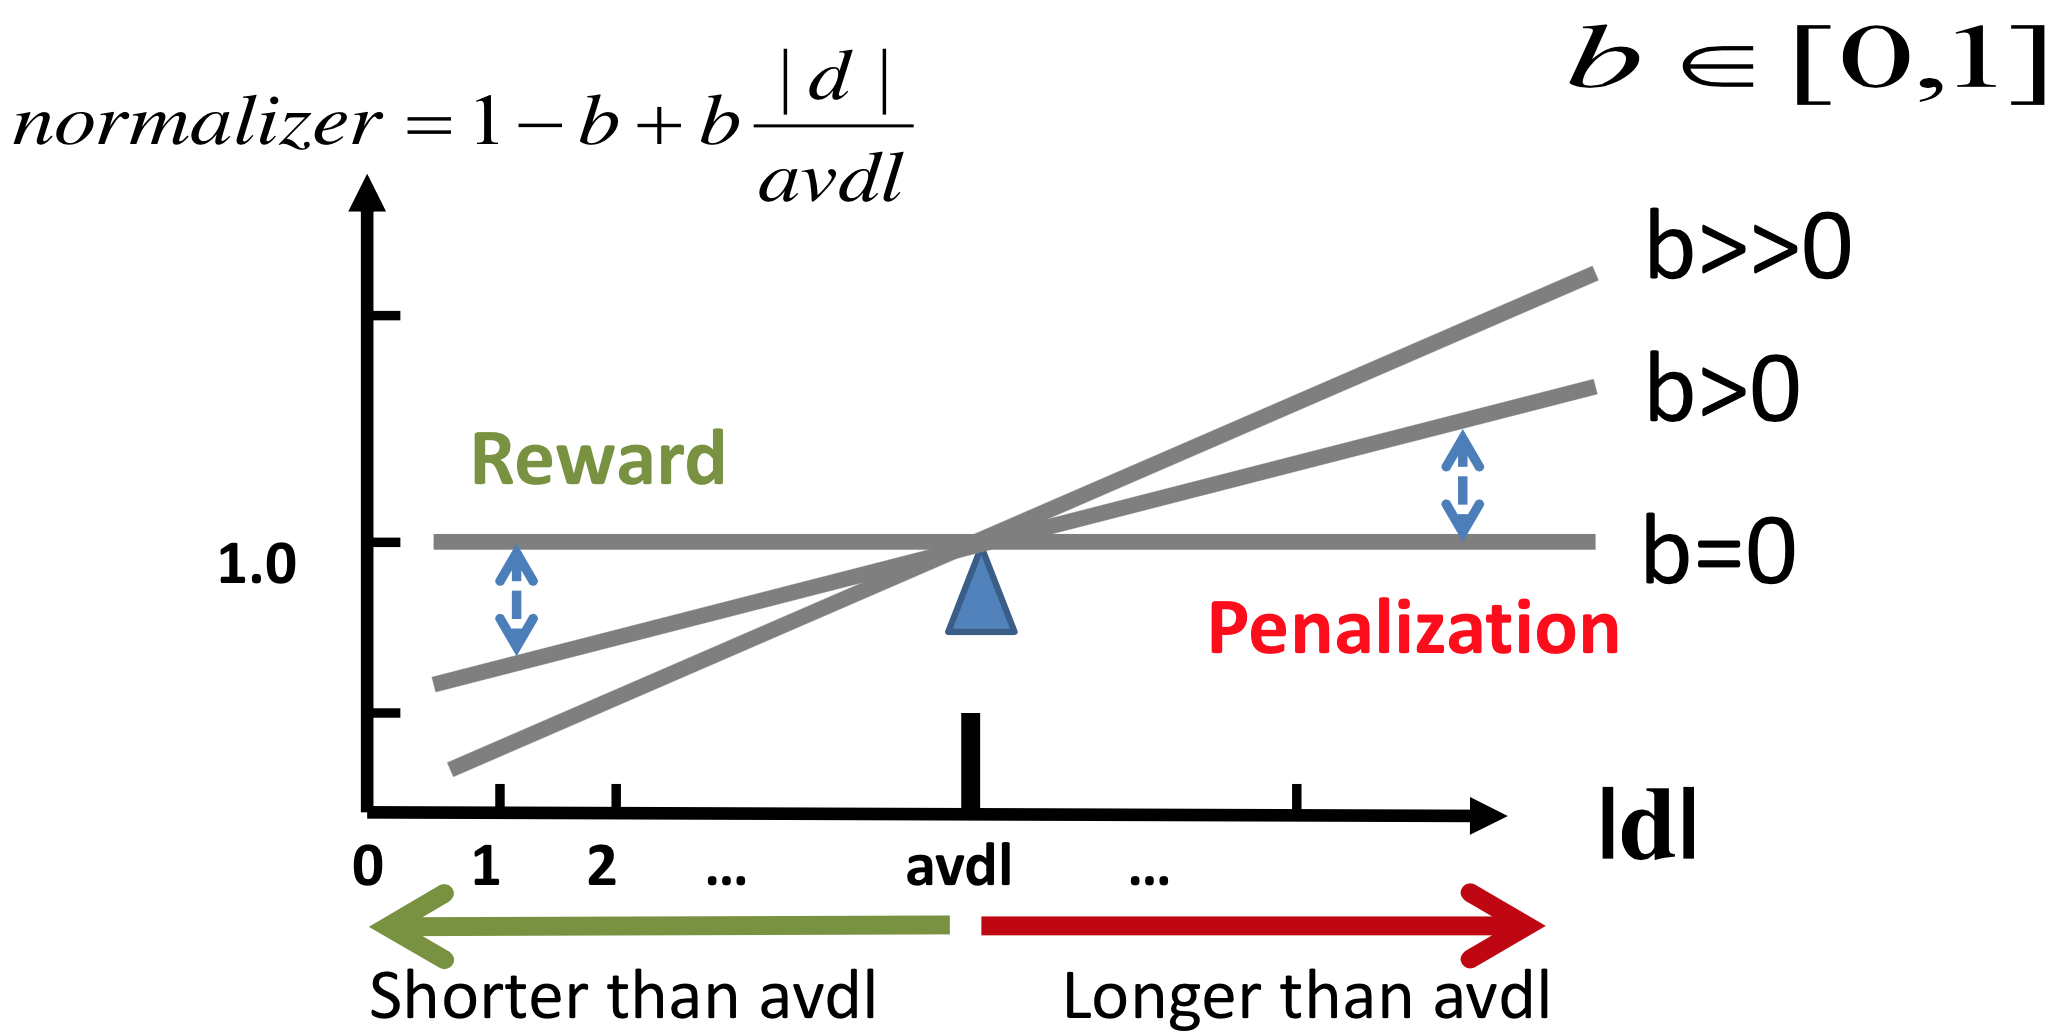
\includegraphics[width=0.75\linewidth]{pivoted_length_norm.png}
\end{figure}


%----------------------------------------
\subsection{State of the Art VSM Ranking Functions}

Pivoted Length Normalization VSM [Singhal et al 96]:
\begin{equation*}
f(q, d) = \sum_{w \in q \cap d} c(w, q) \: \frac{\ln[1+\ln(1+c(w, d))]}{1-b+b\dfrac{|d|}{avdl}} \: \log\frac{M+1}{df(w)}
\end{equation*}


\href{https://ru.wikipedia.org/wiki/Okapi_BM25}{BM25/Okapi} [Robertson \& Walker 94]:
\begin{equation*}
f(q, d) = \sum_{w \in q \cap d} c(w, q) \: \frac{(k+1) \: c(w, d)}{c(w, d) + k\left(1-b+b\dfrac{|d|}{avdl}\right)} \: \log\frac{M+1}{df(w)}
\end{equation*}

%----------------------------------------
\subsection{Further Improvement of VSM?}
\begin{itemize}
\item Improved instantiation of dimension?
\begin{itemize}
\item  stemmed words, stop word removal, phrases, latent semantic indexing (word clusters), character n-grams, ...
\item  bag-of-words with phrases is often sufficient in practice
\item  Language-specific and domain-specific tokenization is important to
ensure “normalization of terms”
\end{itemize}

\item  Improved instantiation of similarity function?
\begin{itemize}
\item  cosine of angle between two vectors?
\item  Euclidean?
\item  dot product seems still the best (sufficiently general especially with appropriate term weighting)
\end{itemize}
\end{itemize}

%----------------------------------------
\subsection{Further Improvement of BM25}
\begin{itemize}
\item BM25F [Robertson \& Zaragoza 09]
\begin{itemize}
\item Use BM25 for documents with structures (<<F>>=fields)
\item Key idea: combine the frequency counts of terms in all fields and then apply BM25 (instead of the other way)
\end{itemize}

\item BM25+ [Lv \& Zhai 11]
\begin{itemize}
\item Address the problem of over penalization of long documents
by BM25 by adding a small constant to TF
\item Empirically and analytically shown to be better than BM25
\end{itemize}
\end{itemize}


%----------------------------------------
\subsection{Summary of Vector Space Model}
\begin{itemize}
\item Relevance(q,d) = similarity(q,d)
\item Query and documents are represented as vectors
\item Heuristic\footnote{Heuristic - эвристический} design of ranking function

\item Major term weighting heuristics 
\begin{itemize}
\item TF weighting and transformation 
\item IDF weighting
\item Document length normalization
\end{itemize}

\item BM25 and Pivoted normalization seem to be most effective
\end{itemize}

\begin{figure}[H]
    \centering
    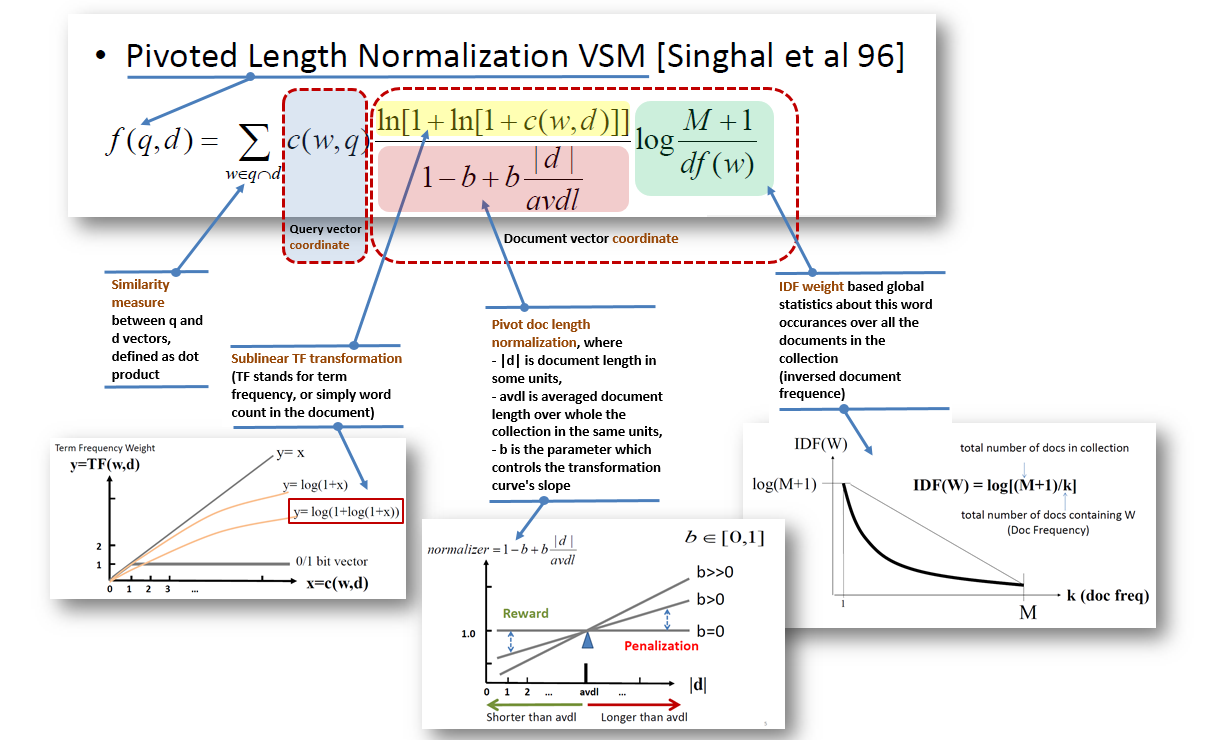
\includegraphics[width=\linewidth]{pivoted_length_normalization_vsm.png}
\end{figure}
\begin{figure}[H]
    \centering
    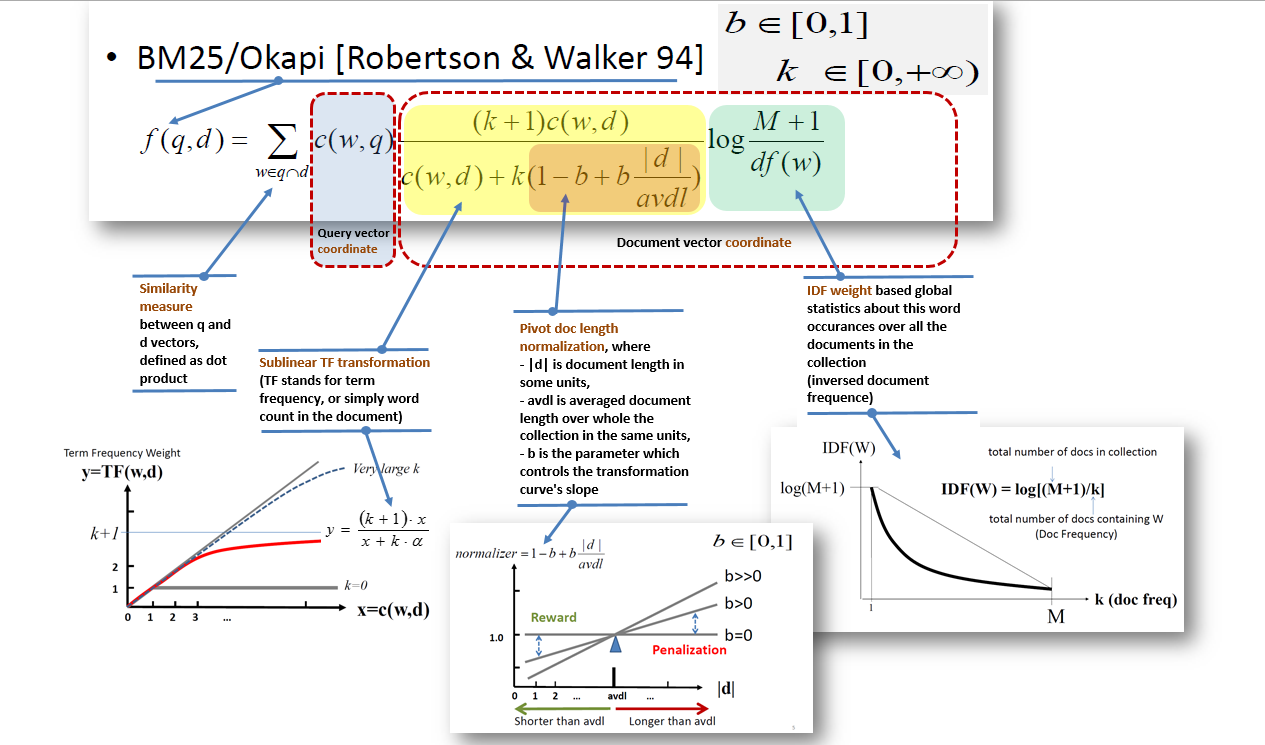
\includegraphics[width=\linewidth]{BM25_Okapi.png}
\end{figure}


%----------------------------------------
\subsection{Recommended reading}
\begin{itemize}
\item A.Singhal, C.Buckley, and M.Mitra. <<Pivoted document length normalization>>. In Proceedings of ACM SIGIR 1996.
\item S. E. Robertson and S. Walker. <<Some simple effective approximations to the 2-Poisson model for probabilistic weighted retrieval>>, Proceedings of ACM SIGIR 1994.
\item S. Robertson and H. Zaragoza. <<The Probabilistic Relevance Framework: BM25 and Beyond>>, Found. Trends Inf. Retr. 3, 4 (April 2009).
\item Y. Lv, C. Zhai, <<Lower-bounding term frequency normalization>>. In Proceedings of ACM CIKM 2011.
\end{itemize}

